\documentclass[12pt]{article}
%-------------PACKAGES-------------%
\usepackage[letterpaper, margin=1.0in]{geometry} % page layout
\usepackage[utf8]{inputenc} % input encoding
\usepackage[T1]{fontenc} % font encoding
\usepackage{parskip} % paragraph formatting
\usepackage{fancyhdr} % header formatting
\usepackage{amsmath} % math features
\usepackage{mathtools} % math formating
\usepackage{amssymb} % math symbols
\usepackage{siunitx} % SI units
\usepackage{graphicx} % images
\usepackage{caption} % captions
\usepackage{multirow} % combine rows in tables
\usepackage{xcolor} % colors
\usepackage[american,straightlabels,nooldvoltagedirection]
{circuitikz} % drawing circuit diagrams
%-------------FORMAT-------------%
\pagestyle{fancy}
\renewcommand{\headrulewidth}{0.5mm}
\renewcommand{\footrulewidth}{0.5mm}
\setlength{\headheight}{14.5pt}
\newcommand{\makeheader}[2]{ % Takes argument {Lab #}{Title}
\begin{center}
\textbf{\huge ECE 230L - \MakeUppercase{#1}}\\~\\
\textbf{\large \MakeUppercase{#2}}\\~\\
\rule{6.5in}{0.5mm}\\
\end{center}
\fancyhead[L]{ECE230L}
\fancyhead[C]{}
\fancyhead[R]{Duke University}
\fancyfoot[L]{Lab Report}
\fancyfoot[C]{#1}
\fancyfoot[R]{Page \thepage}
}
\begin{document}
%------Create header/footer------%
\makeheader{Lab 3}{PN JUNCTION DIODES}
\setcounter{section}{1}
\section{Electrical Characterization of Silicon PN-Junction
Diode}
\begin{itemize}
\item[$\square$] What is the value of the series resistor that
you must choose for the 1N4148 diode (with a 200 mA maximum
current) attached to this 6 V power supply? What will you use in
your circuit?

$R = \frac{V}{I} \therefore R = \frac{6V}{0.2A} = 30\Omega$


\item[$\square$] Create a plot of applied $V_{DC}$ vs. $I_D$ for
this circuit.

\begin{figure}[h]
\centering
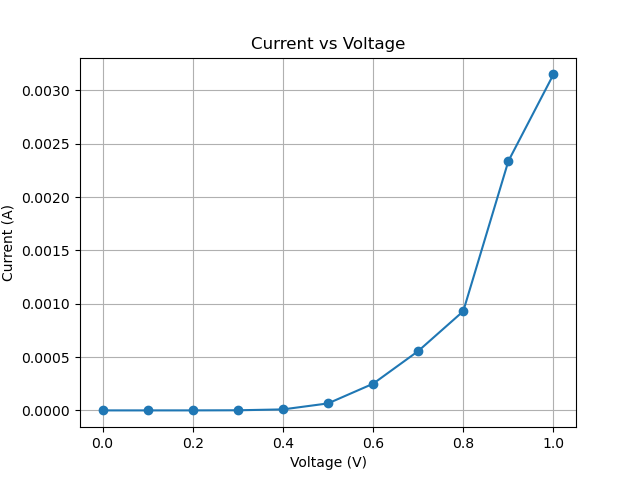
\includegraphics[width=0.8\textwidth]{fig1.png}
\caption{Diode I-V Characteristics}
\label{fig:diode-iv}
\end{figure}

\item[$\square$] What is the knee voltage of the diode in this
circuit?

The knee voltage is the voltage at which the current in the diode begins to increase rapidly.
This is approximately 0.8-0.9V from the manual measurement data.

\item[$\square$] Show the LabVIEW plots for each of the 4
scenarios:
\\
\\

Forward Bias: $I_D(V_{DC})$

\begin{figure}[h!tbp]
    \centering
    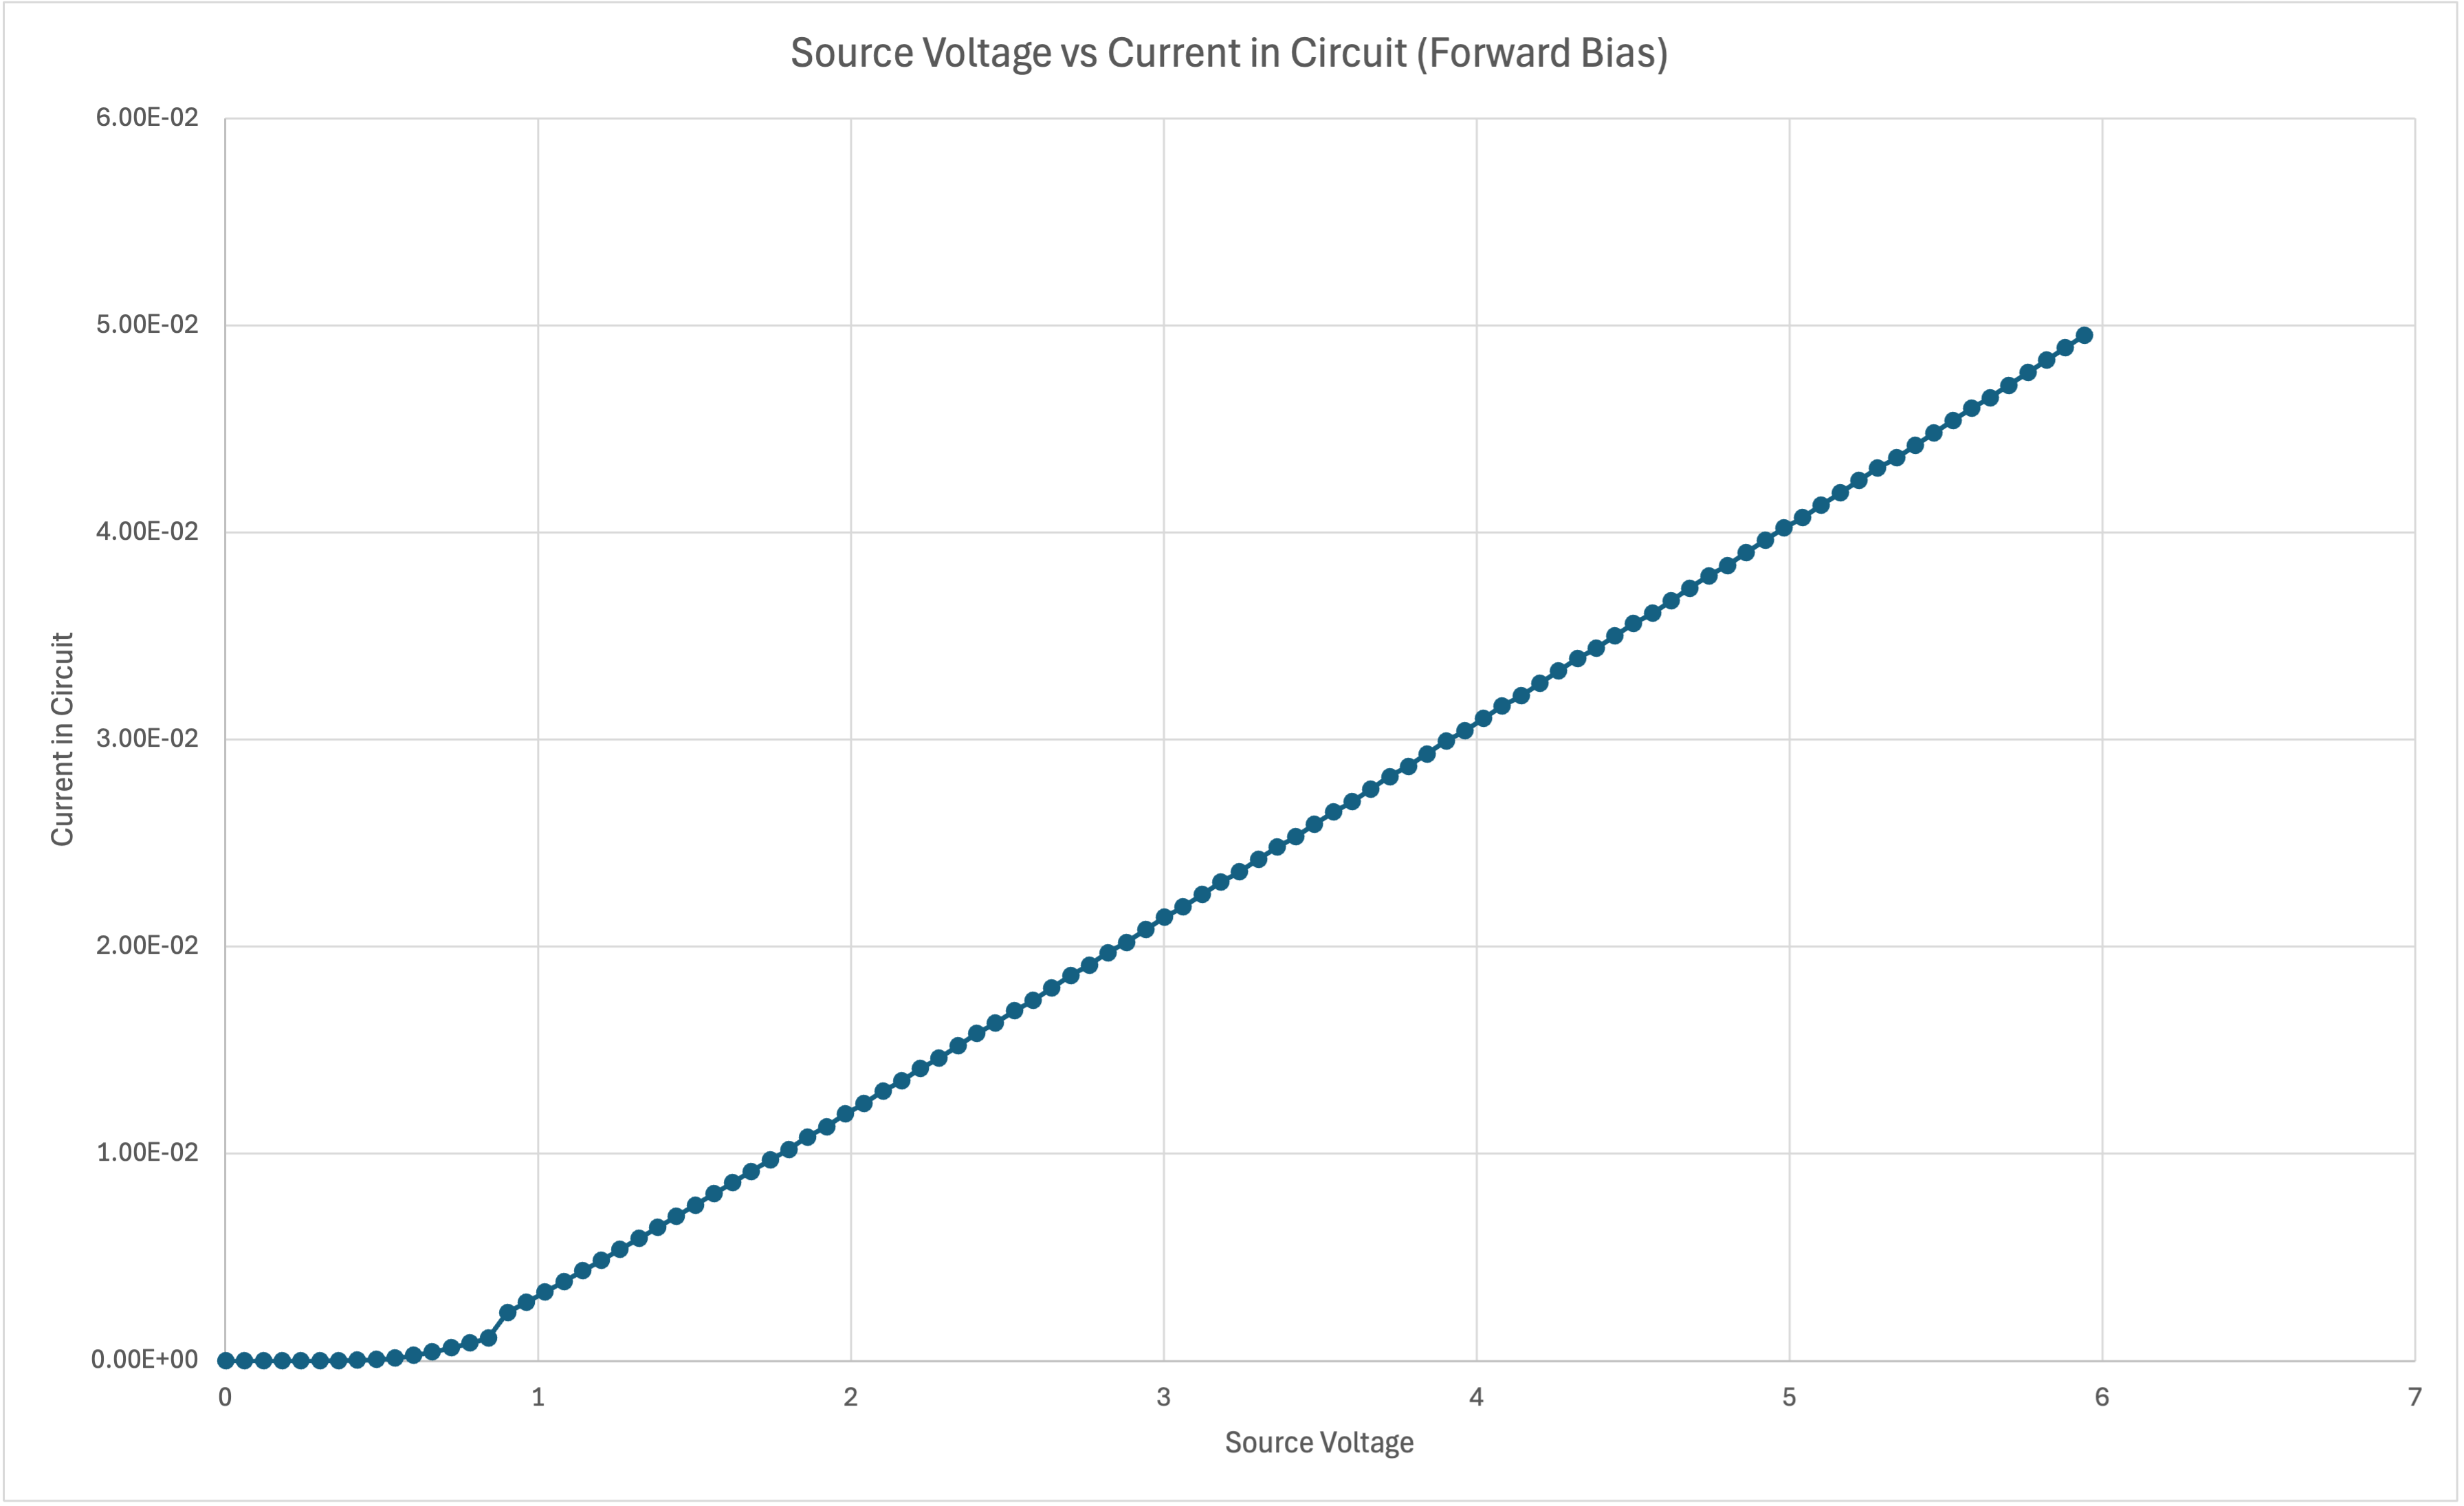
\includegraphics[width=0.8\textwidth]{I_D_forward.png}
    \caption{Forward Bias $I_D(V_{DC})$}
    \label{fig:forward-bias_I}
\end{figure}

Forward Bias: $V_{PN}(V_{DC})$
\begin{figure}[h!tbp]
    \centering
    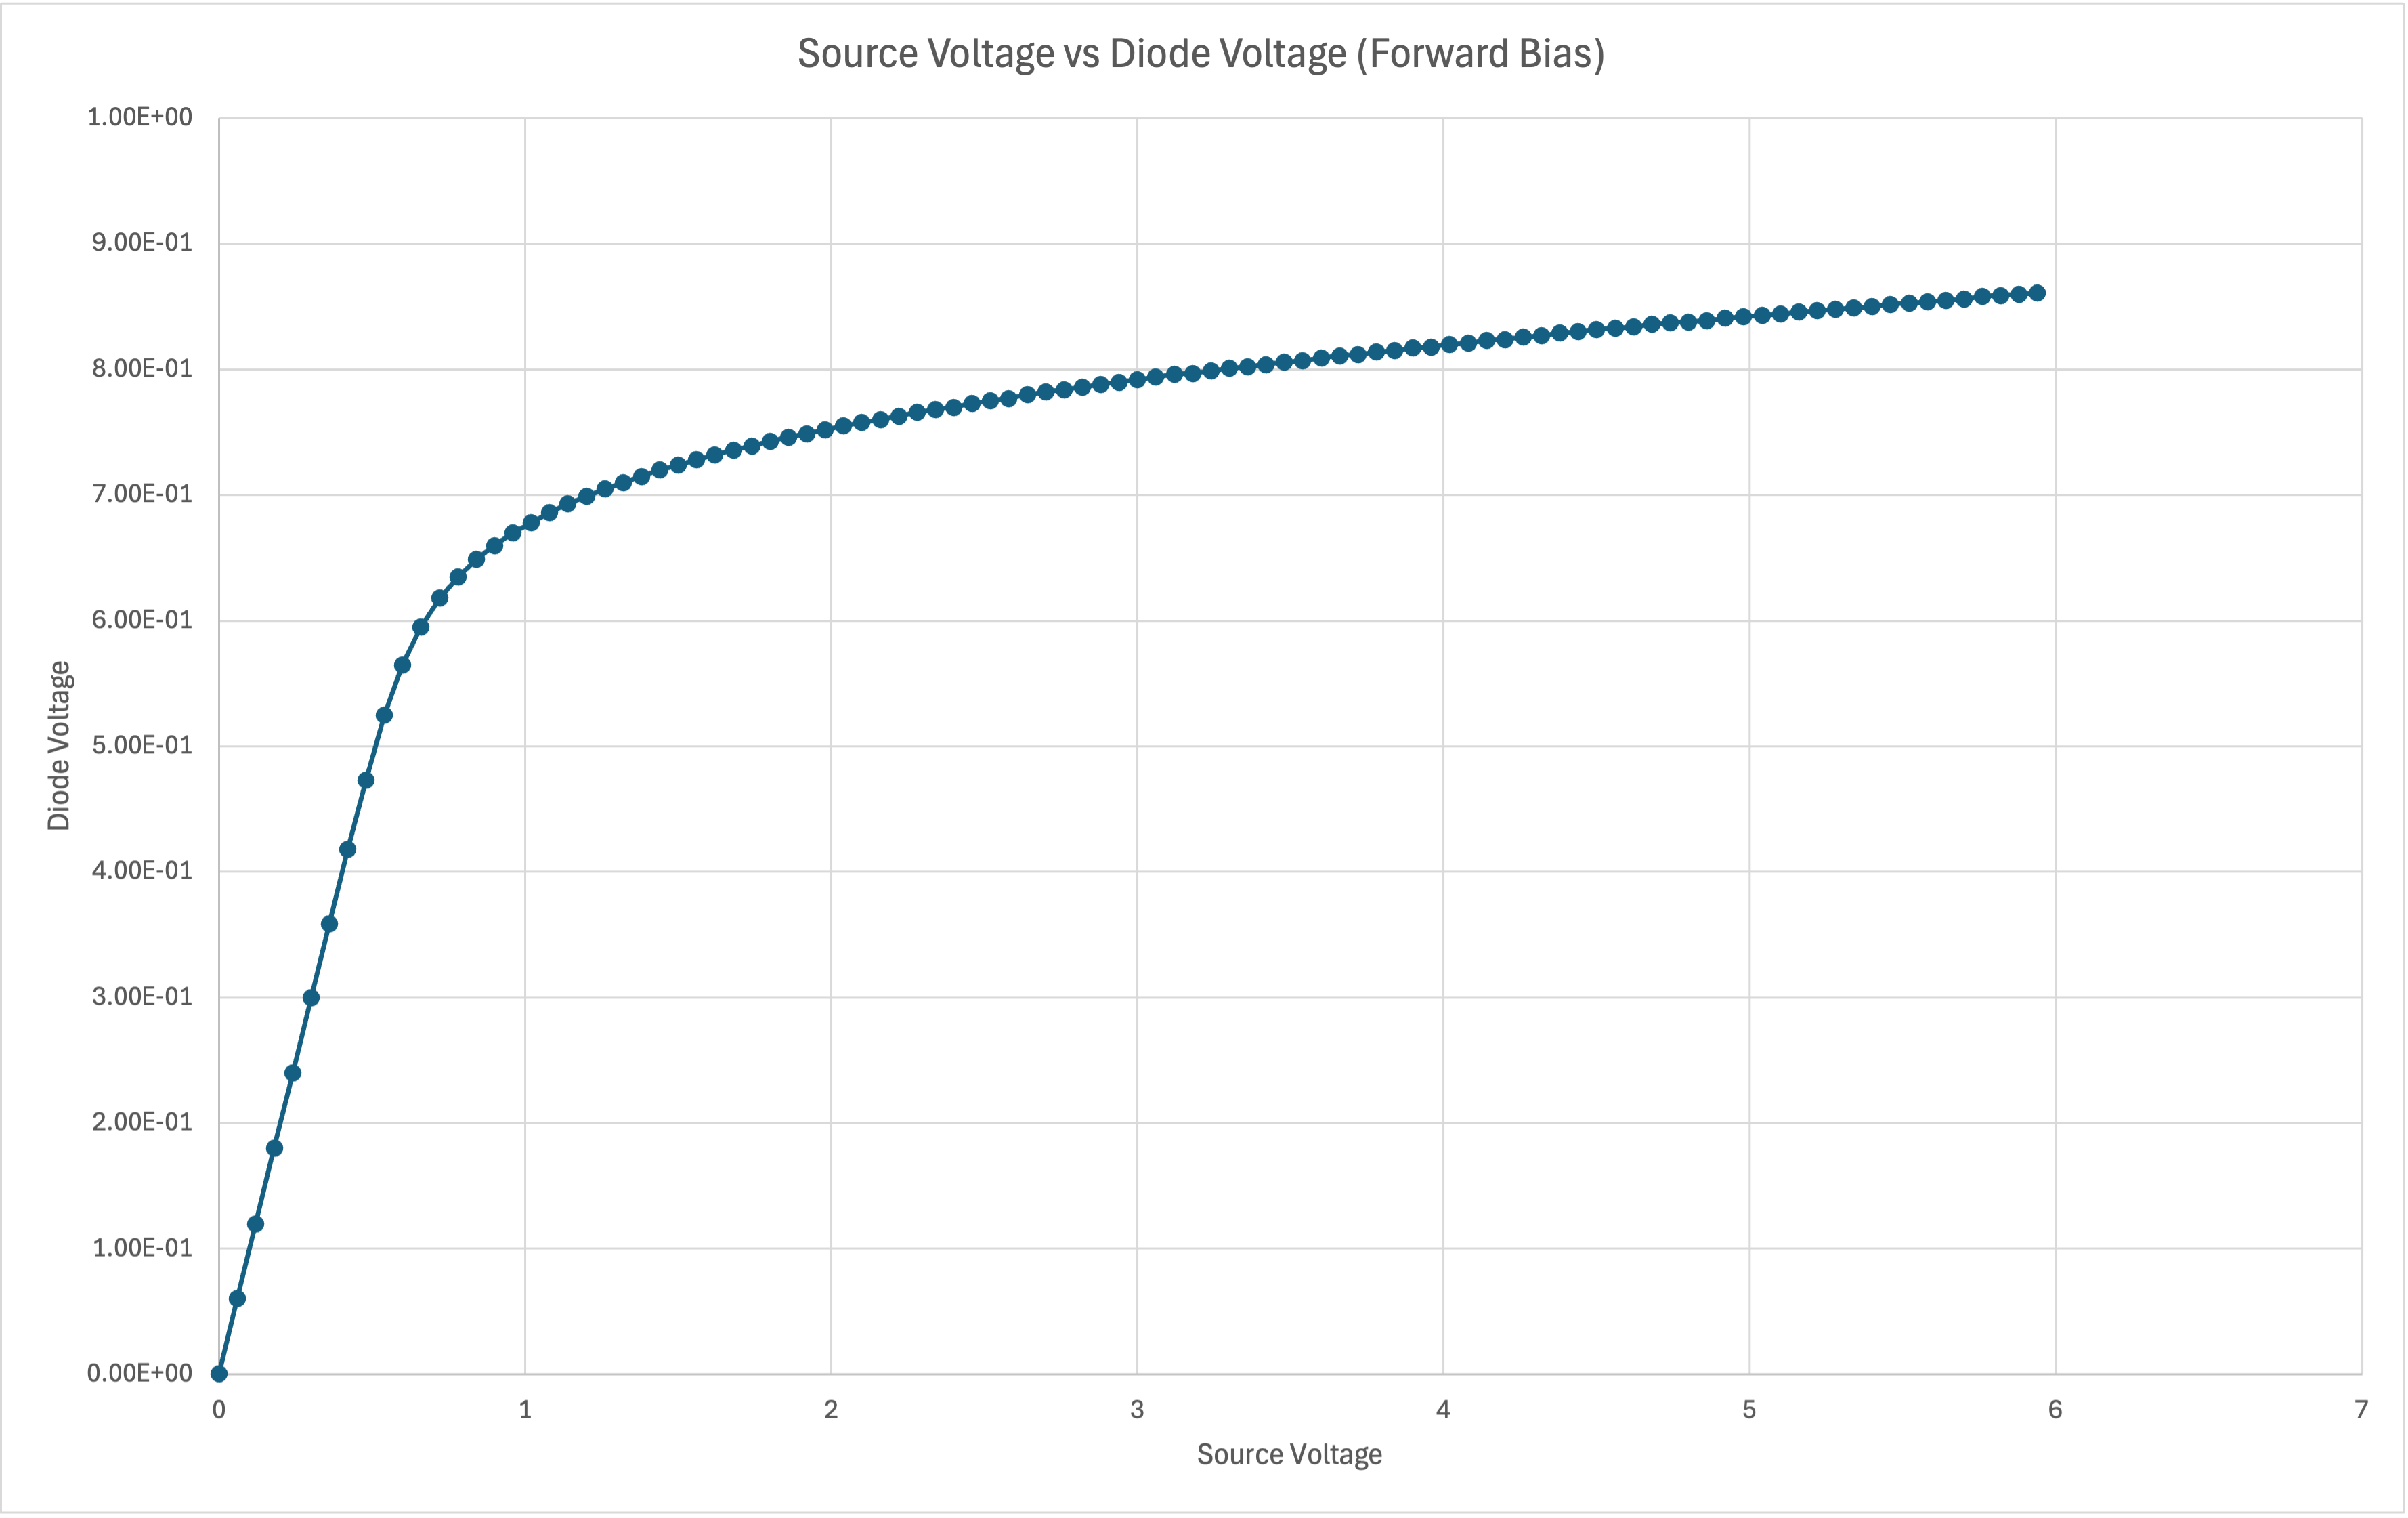
\includegraphics[width=0.8\textwidth]{V_PN_forward.png}
    \caption{Forward Bias $V_{PN}(V_{DC})$}
    \label{fig:forward-bias_V}
\end{figure}

\newpage

Reverse Bias: $I_D(V_{DC})$
\begin{figure}[h!tbp]
    \centering
    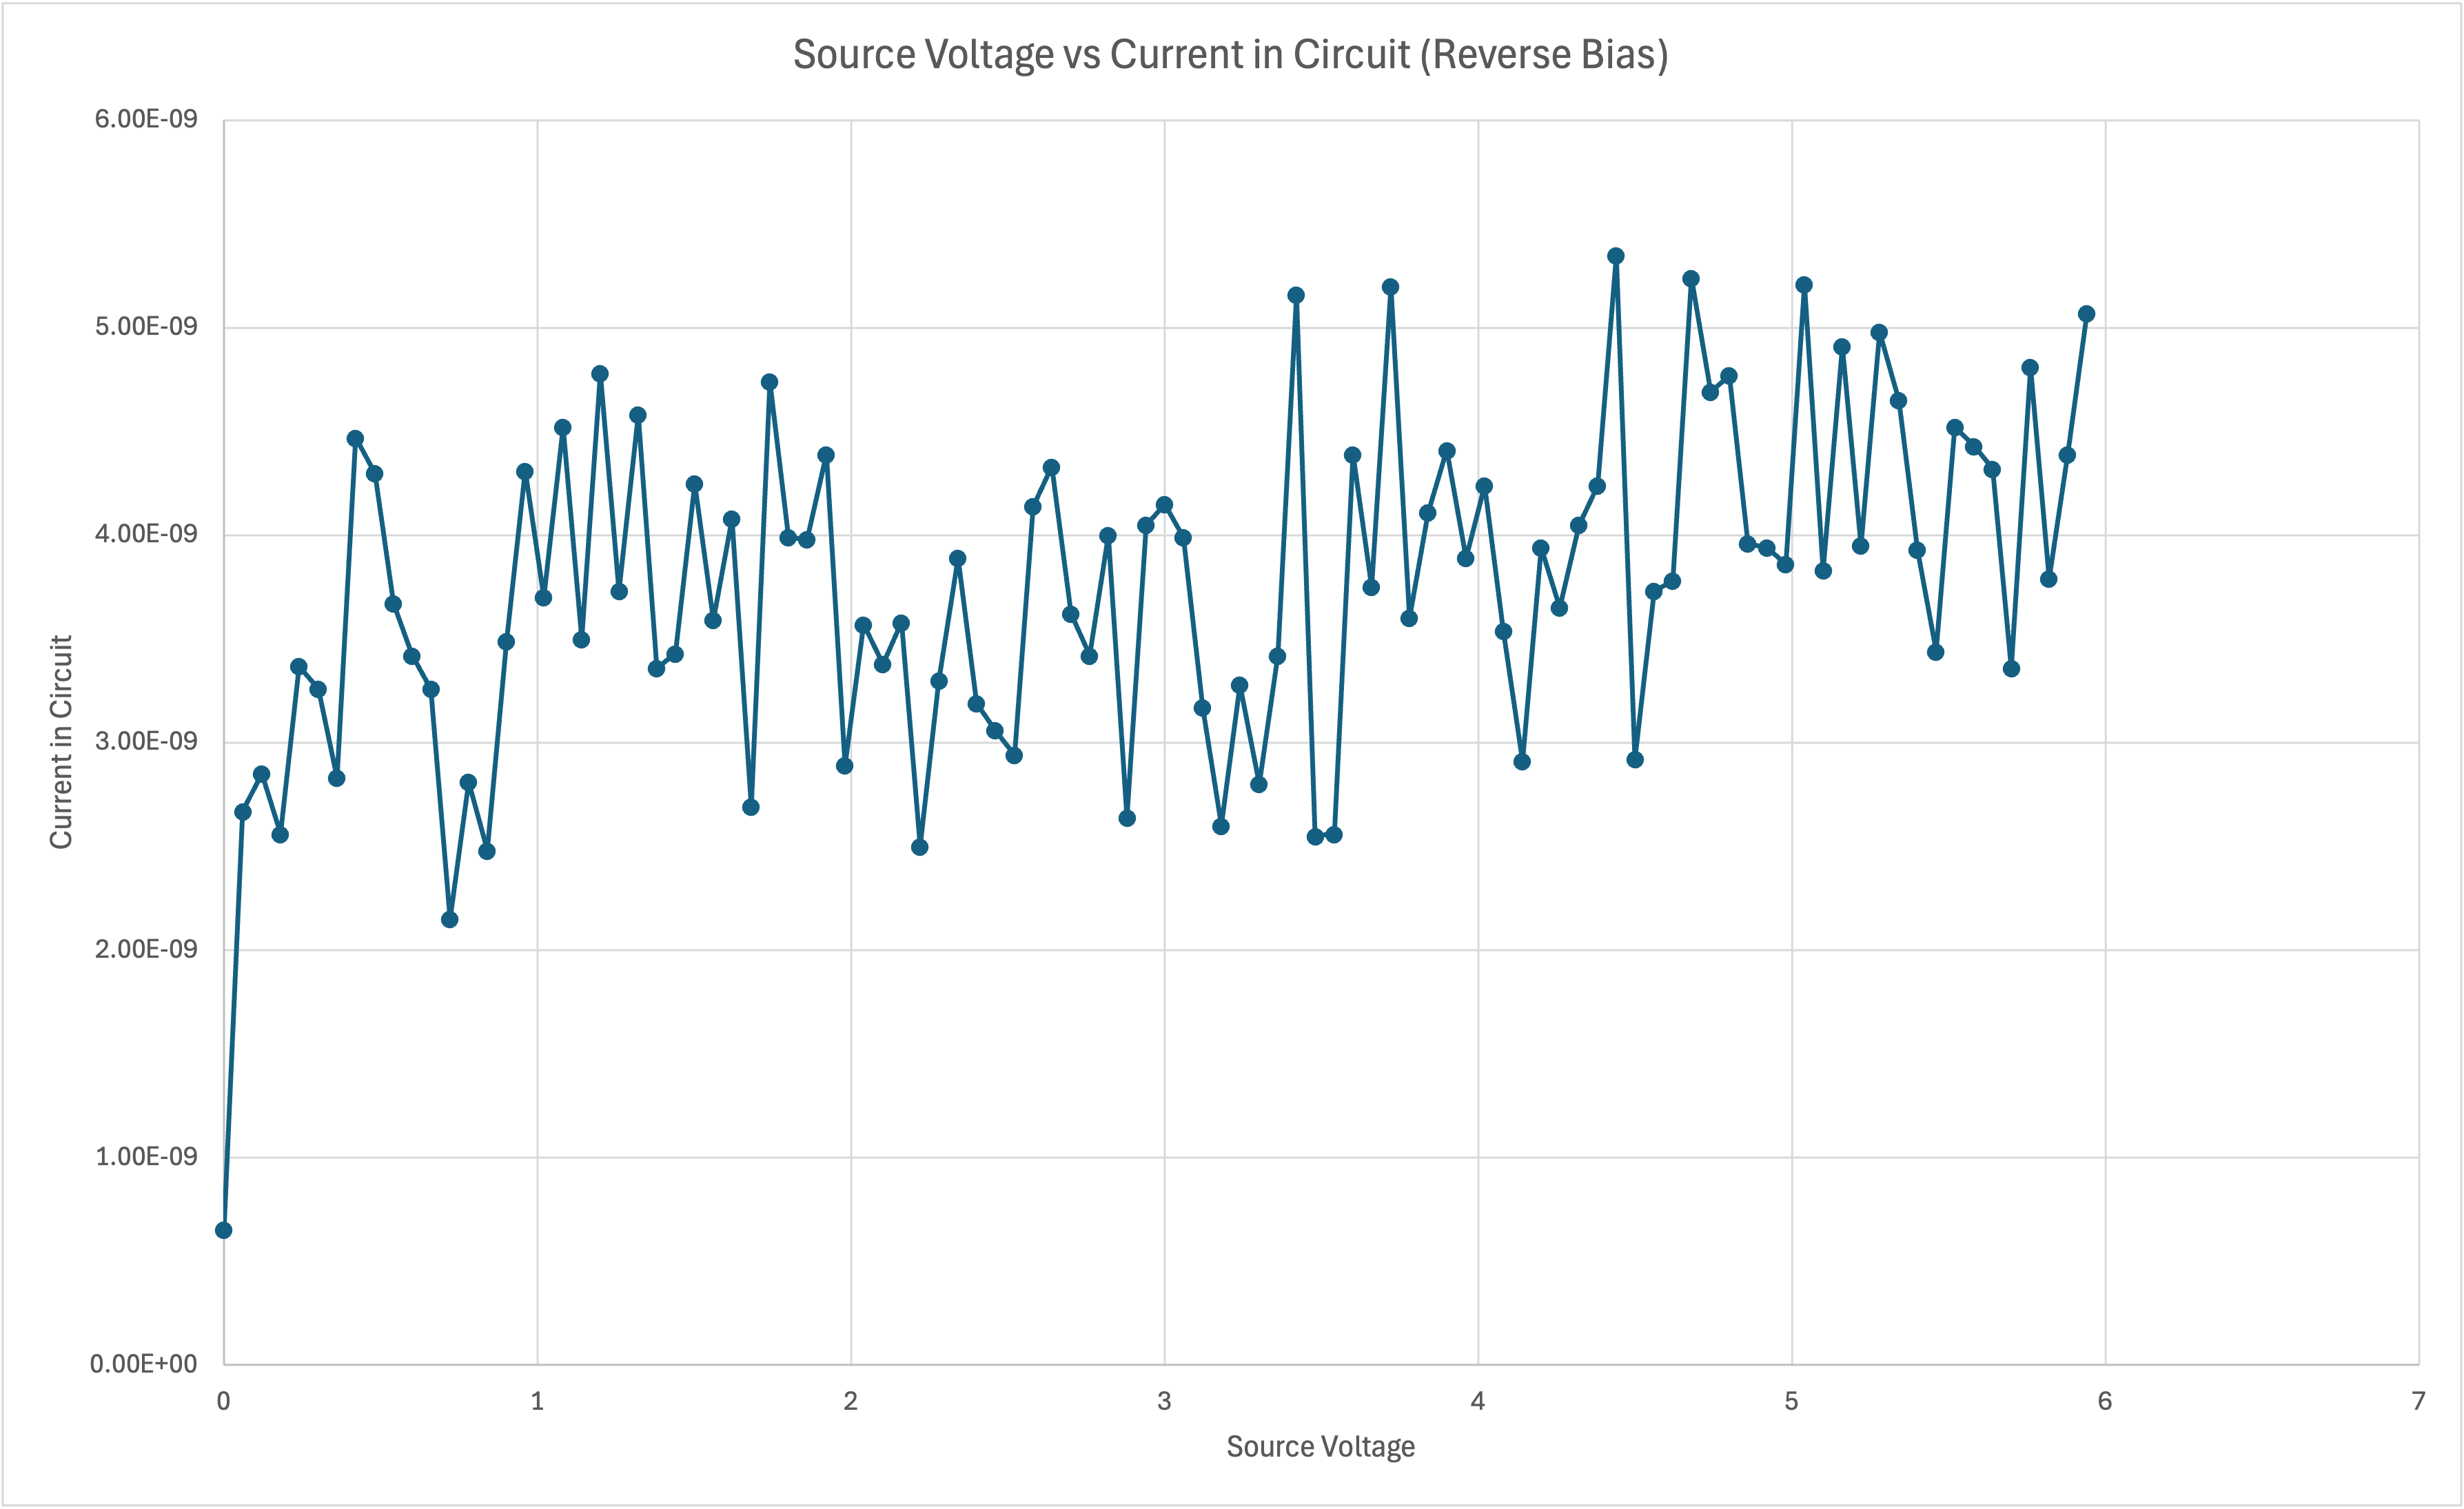
\includegraphics[width=0.8\textwidth]{I_D_reverse.png}
    \caption{Reverse Bias $I_D(V_{DC})$}
    \label{fig:reverse-bias_I}
\end{figure}

Reverse Bias: $V_{PN}(V_{DC})$
\begin{figure}[h!tbp]
    \centering
    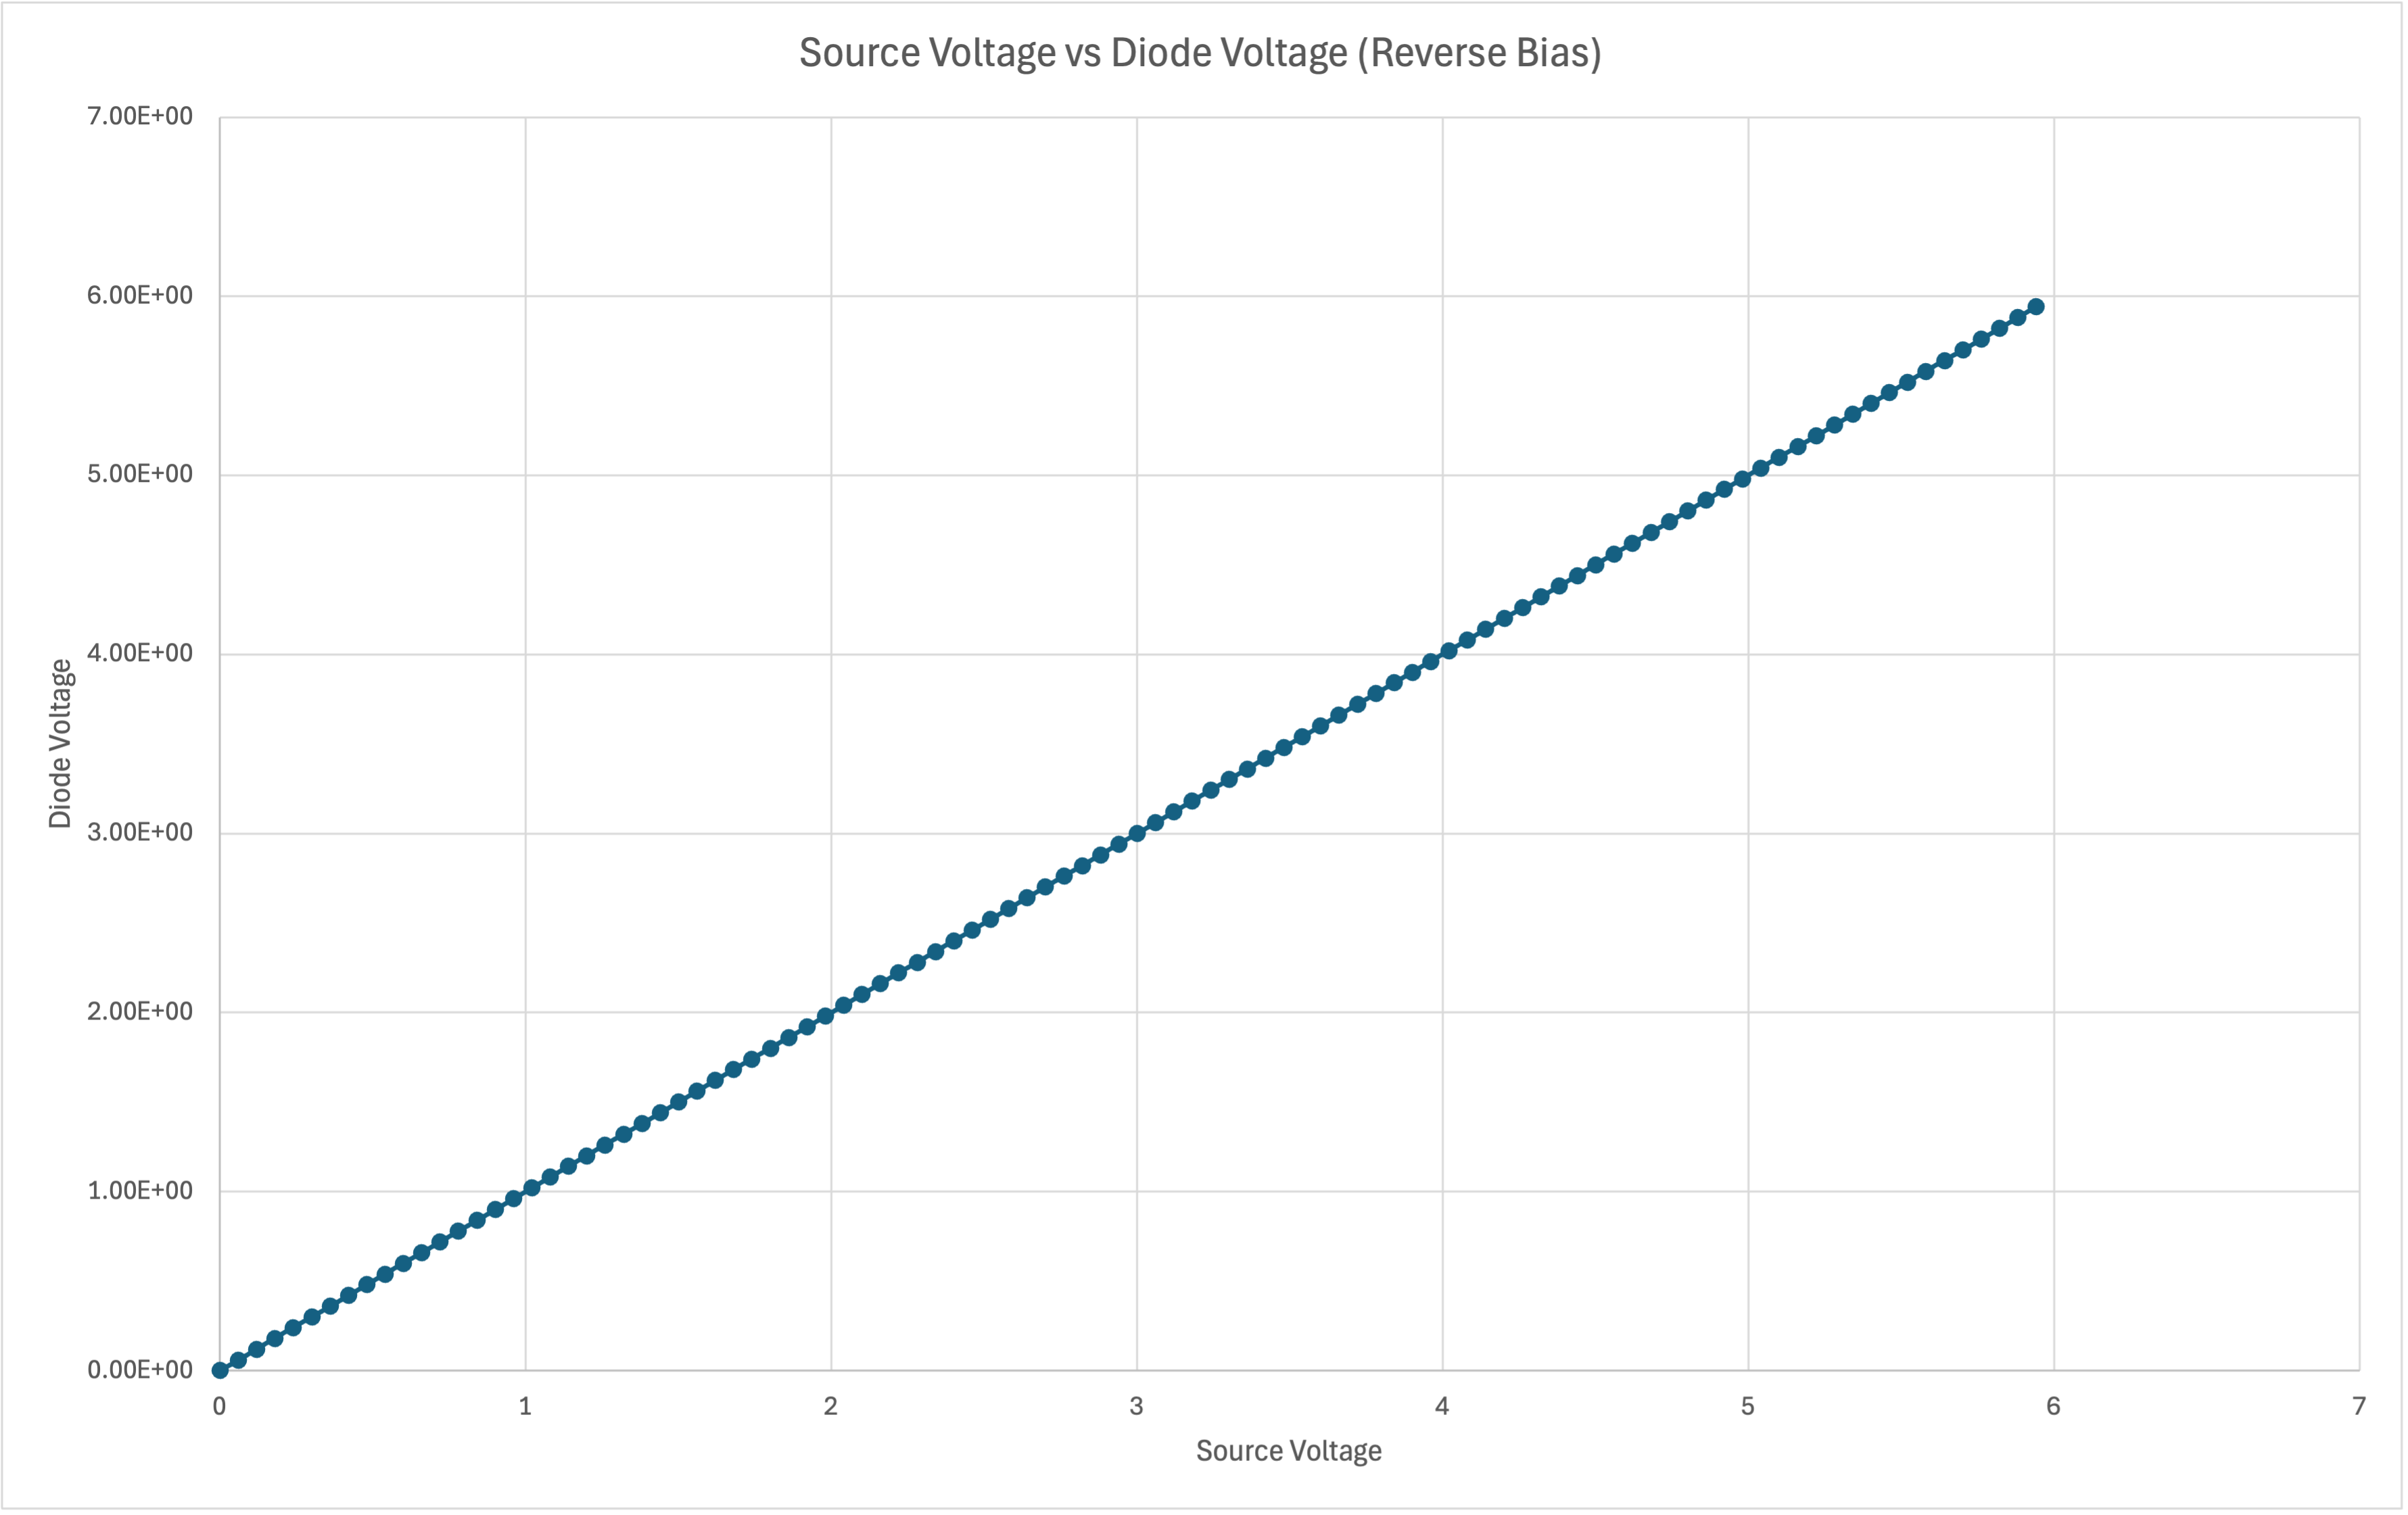
\includegraphics[width=0.8\textwidth]{V_PN_reverse.png}
    \caption{Reverse Bias $V_{PN}(V_{DC})$}
    \label{fig:reverse-bias_V}
\end{figure}
    

\end{itemize}
\newpage
\newpage
\section{Explorations}
\subsection{PN-Junction Diode Half-Wave and Bridge Rectifiers}
\subsubsection*{Half-Wave Rectifier}
\begin{itemize}
\item[$\square$]{\label{item1}} Capture of the oscilloscope
screen
\begin{figure}[h]
\centering
% \includegraphics[width=0.7\textwidth]{}
\caption{Half-Wave Rectifier}
\label{fig:half-wave}
\end{figure}
\item[$\square$]{\label{item2}} Measure the peak voltage from the
ground reference (GND or 0 V) on the oscilloscope screen to V$_{\
mathrm{peak}}$ of the rectified waveform. What do you notice about
the maximum voltage of the rectified waveform? Is it greater than
or smaller than the maximum peak voltage of the input waveform?
What is the difference in Volts? Is this difference value a
characteristic of the diode behavior?
\item[$\square$] Observe the output waveform with the capacitor
added. What has happened? How could this circuit be useful?
\end{itemize}
\subsubsection*{Bridge Rectifier}
\begin{enumerate}
\item[$\square$] Capture of the oscilloscope screen
\begin{figure}[h]
\centering
% \includegraphics[width=0.7\textwidth]{}
\caption{Bridge Rectifier}
\label{fig:half-wave}
\end{figure}
\item[$\square$] Measure the amplitude of this rectified waveform.
Compare the amplitude of the rectified waveform of the Bridge
Rectifier to the amplitude of the rectified waveform in the Half-
Wave Rectifier. What do you notice about the amplitude of the
Bridge Rectifiers rectified waveform? Why?
\end{enumerate}
\newpage
\subsection{LED Lighting}
\begin{enumerate}
\begin{table}[h]
\def\arraystretch{1.5}
\centering
\begin{tabular}{|c|c|c|c|}
\hline
& Power Draw & Current Flow & \def\arraystretch{1}\begin{tabular}{@{}c@{}}Distance between\\light and photoresistor\end{tabular} \\\hline
Incandescent Light Bulb & 58.7 W& 68.2 $\mu$A & 0.05m\\\hline
LED Light Bulb & 9.5 W & 10.8 $\mu$A & 0.05m\\\hline
\end{tabular}
\caption{LED lighting measurements}
\label{tab:led-lighting}
\end{table}
\item[$\square$] Give a brief explanation of your findings.
Comment on the pros and cons of the LED and incandescent light
bulbs considering the following:
\begin{itemize}
\item Brightness (qualitative and quantitative), Power, Power
efficiency, Color

From the comparison between the incandescent and LED light bulbs, several observations can be made. 

In terms of power consumption, the incandescent light bulb draws significantly more power (58.7 W) compared to 
the LED light bulb (9.5 W). This clearly shows that LEDs are much more power-efficient. Despite this lower power 
consumption, the current flow in the incandescent bulb (68.2 $\mu$A) is also higher than that in the LED (10.8 $\mu$A), 
further supporting the fact that LEDs are more efficient in converting electrical energy into light output.

Despite the lower power draw, LEDs often provide similar or 
even better brightness compared to incandescent bulbs, as they seem to produce light without 
generating nearly as much heat. The LEDs also seemed to produce cooler light, while the bulb emitted a warmer, 
yellowish light.

Overall, LEDs offer significant advantages in terms of power efficiency and longevity, but the warmer color 
and even the heating aspect of incandescent bulbs can still be appealing in certain lighting situations.
\end{itemize}
\end{enumerate}
\newpage
\subsection{Colored LEDs}
Create forward-biased I-V curves for the Red, Yellow, and Green
LEDs available in lab, and plot them on the same graph as the
Silicon 1N4148 diode measured in the laboratory exercise above.
\begin{figure}[h]
\centering
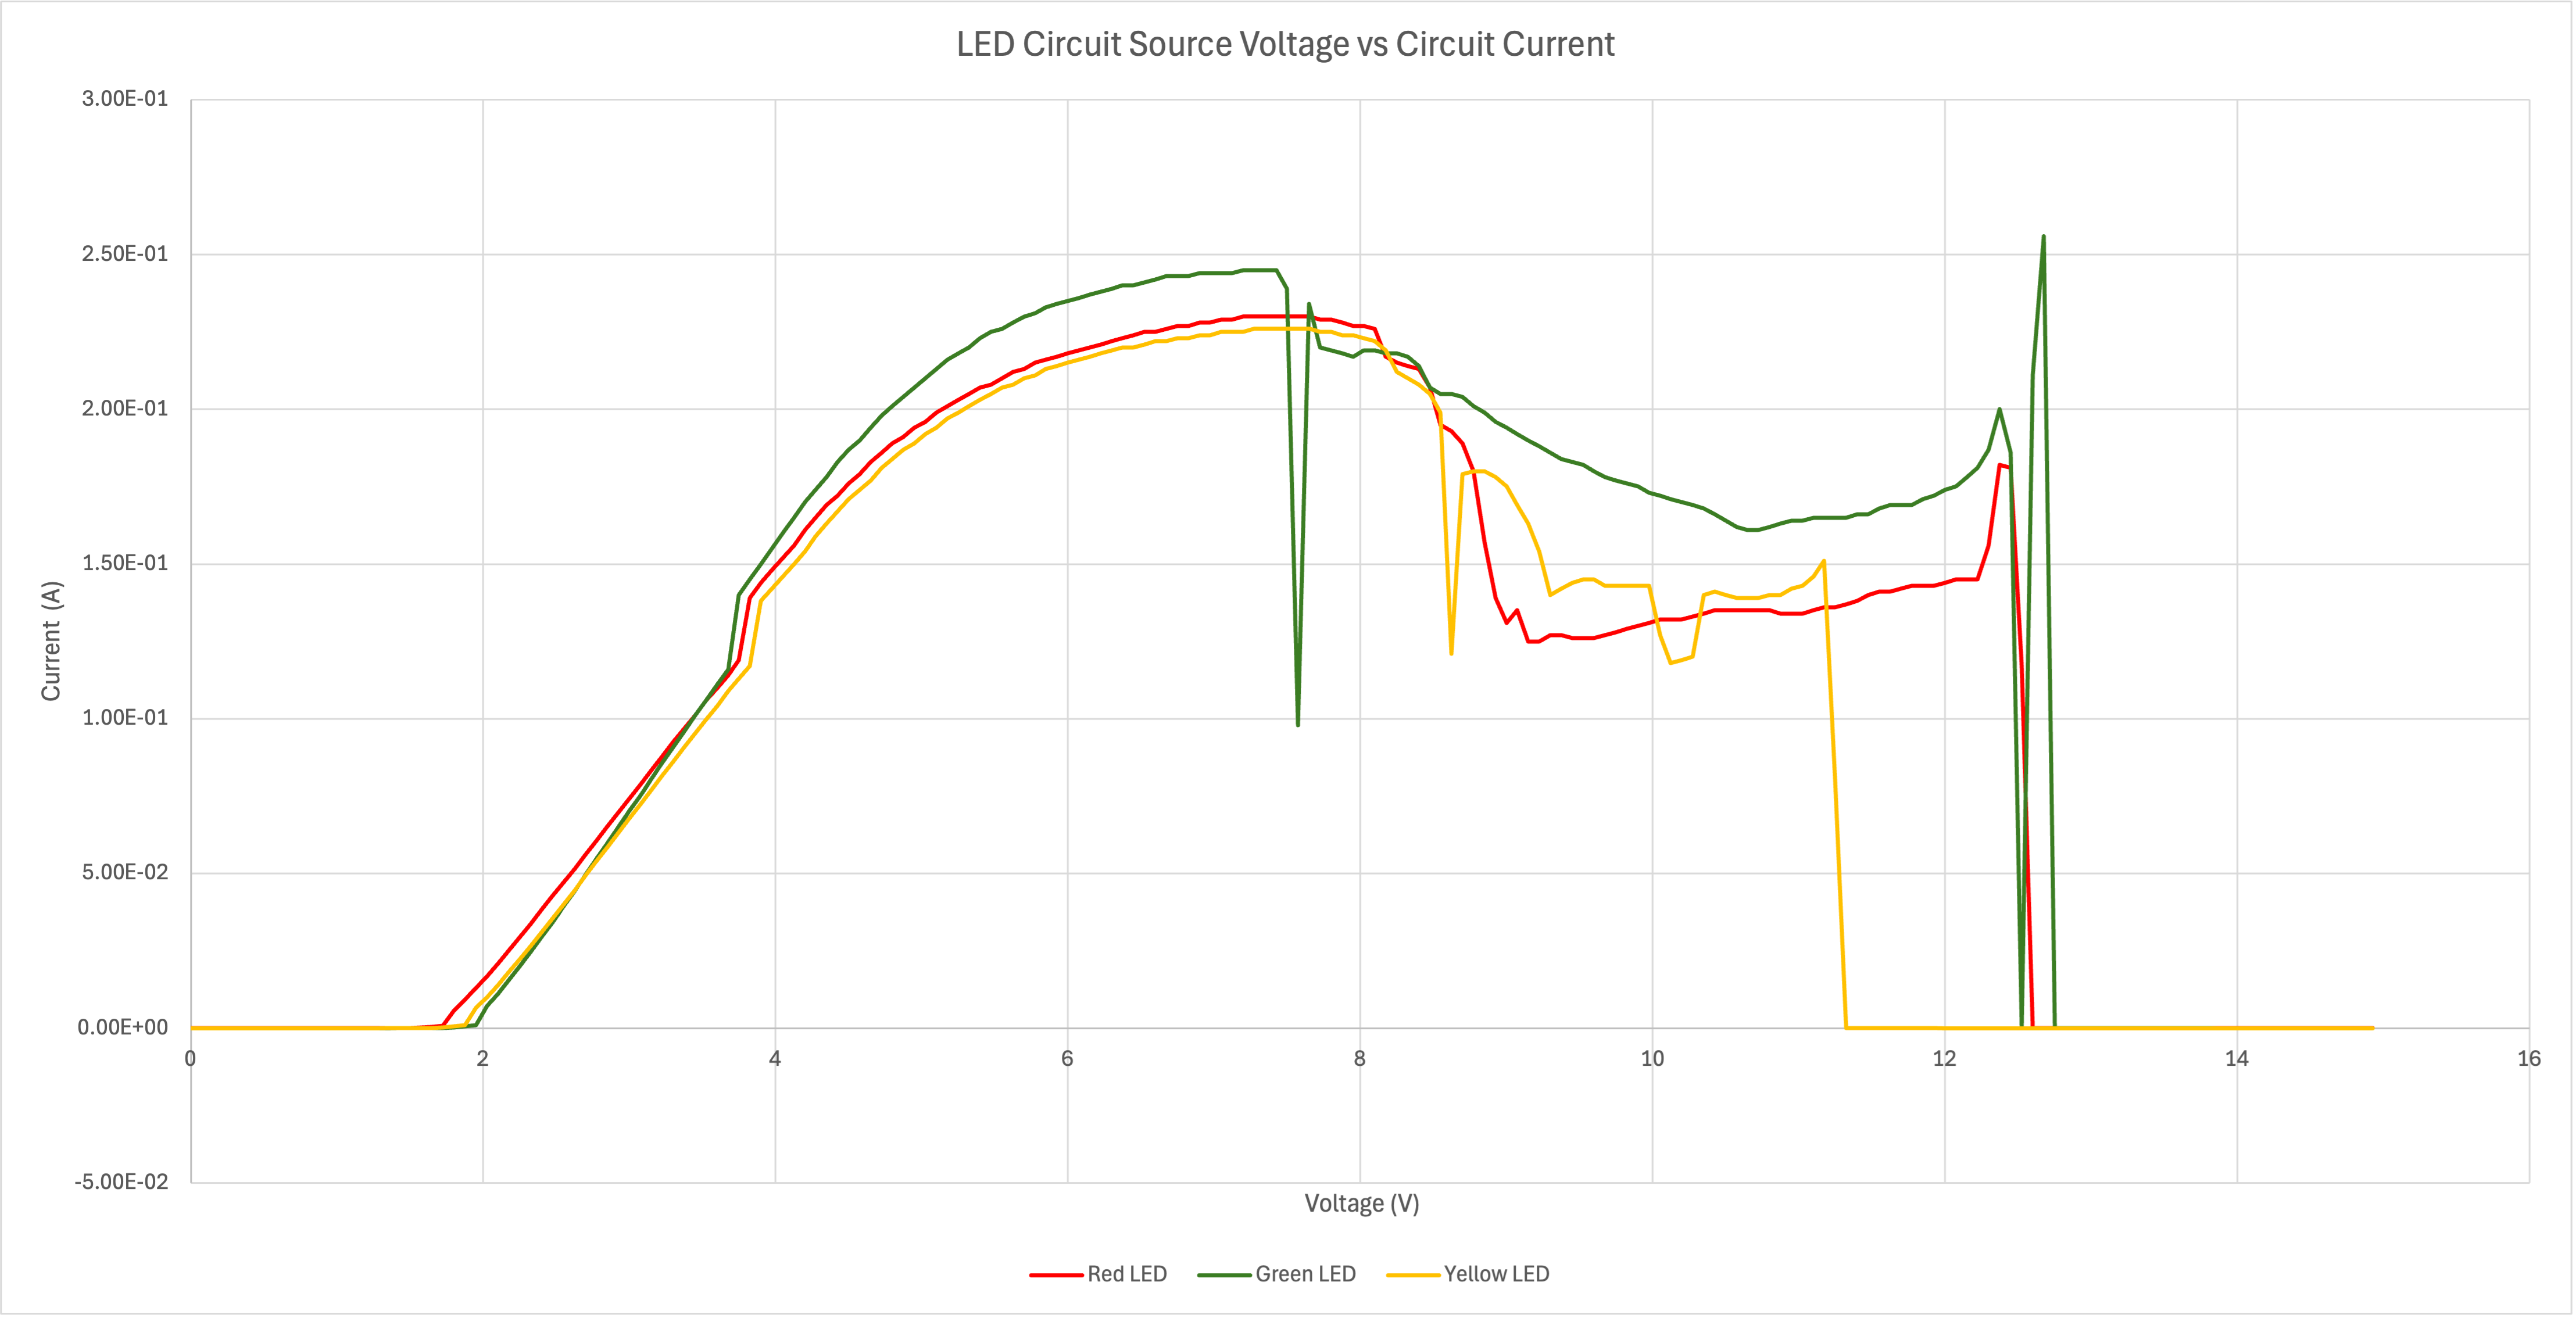
\includegraphics[width=0.95\textwidth]{LED_Circuit.png}
\caption{Colored LED I-V Curves}
\label{fig:colored-leds}
\end{figure}
For each of the LEDs, determine the following:
\begin{itemize}
\item[$\square$] the knee voltage where the diode turns on

Red: 1.8V, Green: 2.0V, Yellow: 1.9V
\newpage

\item[$\square$] the saturation current, $I_S$
\begin{figure}[h]
    \centering
    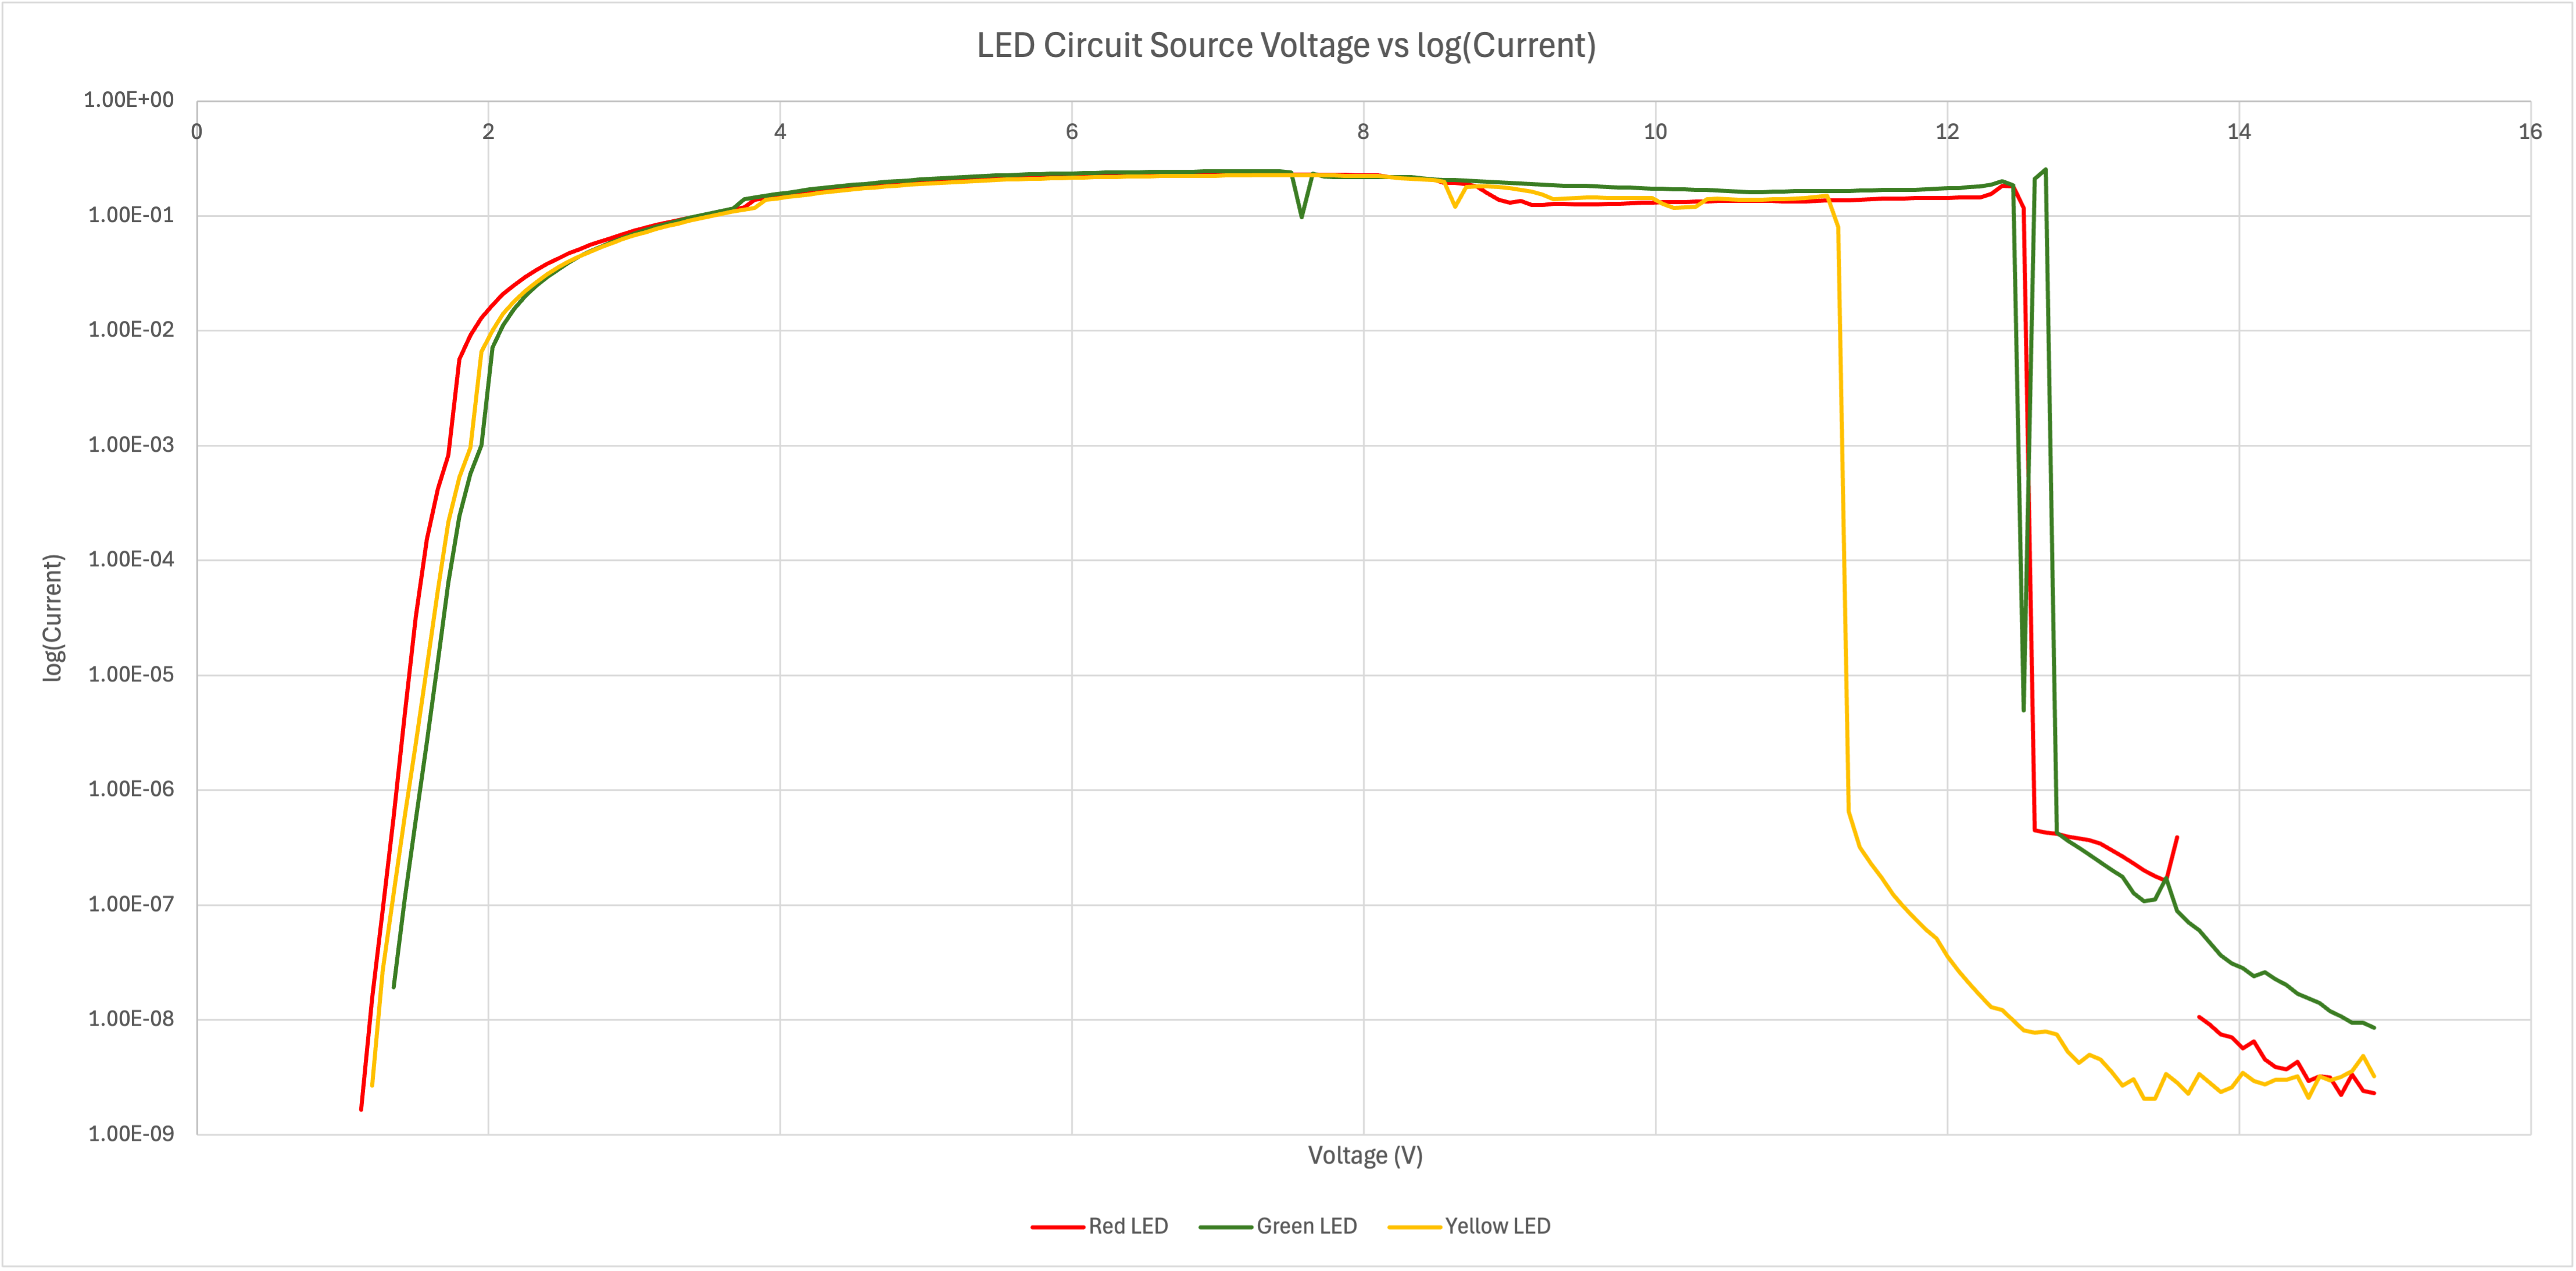
\includegraphics[width=0.95\textwidth]{log_LED.png}
    \caption{Colored LED log(I)-V Curves}
    \label{fig:colored-leds-2}
\end{figure}

$\therefore$ saturation current is the intercept.
All LEDs have the saturation current gradient around 2.8-3.6V. \\
Intercepts: \\
Red ~ 0.01A,
Green ~ 0.01A,
Yellow ~ 0.01A

\item[$\square$] the ideality factor, $n$

$n = \frac{V_{PN.2} - V_{PN.1}}{\frac{k_B T}{q} \ln\left(\frac{I_D(V_{PN.2})}{I_D(V_{PN.1})}\right)}$

Straight line region is between 2.8-3.6V. \\

$\therefore V_{PN.1} = 2.8V, V_{PN.2} = 3.6V$ \\
$I_D(V_{PN.1}) = 0.07A, I_D(V_{PN.2}) = 0.1A$ \\

$T = 300K, k_B = 1.38 \times 10^{-23} J/K, q = 1.6 \times 10^{-19} C$ \\

$\therefore n = \frac{3.6 - 2.8}{\frac{1.38 \times 10^{-23} \times 300}{1.6 \times 10^{-19}} \ln\left(\frac{0.1}{0.07}\right)} = 86.68$

\item[$\square$] the series resistance, $R_S$

Red: 2.8$M\Omega$, Green: 3.0$M\Omega$, Yellow: 2.6$M\Omega$

\item[$\square$] the current at which the LED begins to become
damaged

Red: 12.4A, Green: 12.5A, Yellow: 11.2A

\item[$\square$] the voltage and current when the LED completely
stops functioning (i.e. blow it up---this may require as much as
15V)

Red: 12.7V, 0.175A, Green: 12.9V, 0.25A, Yellow: 11.3V, 0.15A
\end{itemize}
\newpage
\setcounter{section}{4}
\section{Questions}
\begin{enumerate}
\item Define all parameters and variables in Equation (1).

$I_D$ = current through the diode,

$V_{PN}$ = voltage across the PN junction,

$I_S$ = saturation current - the maximum current that can flow through the diode before it is damaged,

$q$ = charge of an electron,

$\gamma$ = ideality factor,

$k_B$ = Boltzmann constant,

$T$ = temperature in Kelvin

\item Plot the $I_D(V_{PN})$ characteristics obtained using
LabVIEW on a log-linear plot. Note that the term `log-linear' is
used to describe a semi-log plot with a logarithmic scale on the
y-axis and a linear scale on the x-axis. The y-axis label should
read `1N4148 Diode Current, $I_D$ (A)' and the x-axis label
should read `Diode Voltage, $V_{PN}$ (V).' Make sure to have
enough data points to generate a smooth curve. Use the measured
value of $V_{PN}$ (from your $V_{PN}$ vs $V$ plot) across the
diode in this plot, i.e., do not assume that the voltages
supplied by the power supply are those across the diode.


\begin{figure}[h]
    \centering
    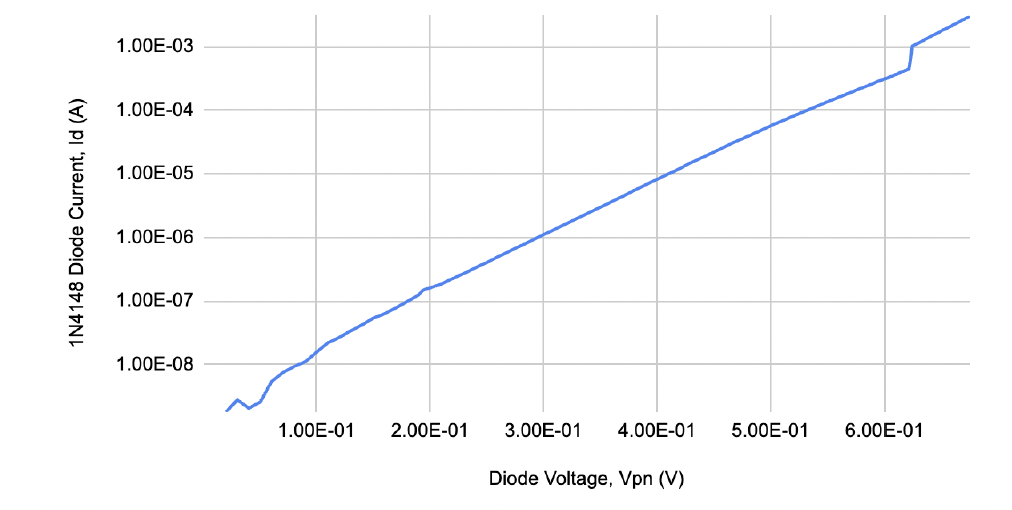
\includegraphics[width=0.95\textwidth]{q1_plot.png}
    \caption{}
    \label{fig:colored-leds-22}
\end{figure}


\item From the above log-linear plot of the I-V characteristics
of the 1N4148, determine the saturation current, $I_S$, the
ideality factor, $n$, and the series resistance, $R_S$. (Refer to
the slides on Canvas for parameter extraction.) For reference,
the values obtained by the TA are $I_{S} = 4*10^{-9}A$, $n =
1.82$, and $R_{S} = 1.40 \Omega$.

$I_S$ = 6.2 * 10-9 A

Using equation (2), the ideality factor, $n$, is 1.95

At the knee voltage, the series resistance, $R_S$, is 1.2 $\Omega$

\item To the above plot from Question 2, add the theoretical PN-
junction diode $I_D(V_{PN})$ characteristic curve. Use the
parameters calculated in Question 3. Vary the parameters, if
necessary, to match the \textbf{log-linear} portion of the
experimentally measured data.

\begin{figure}[h]
    \centering
    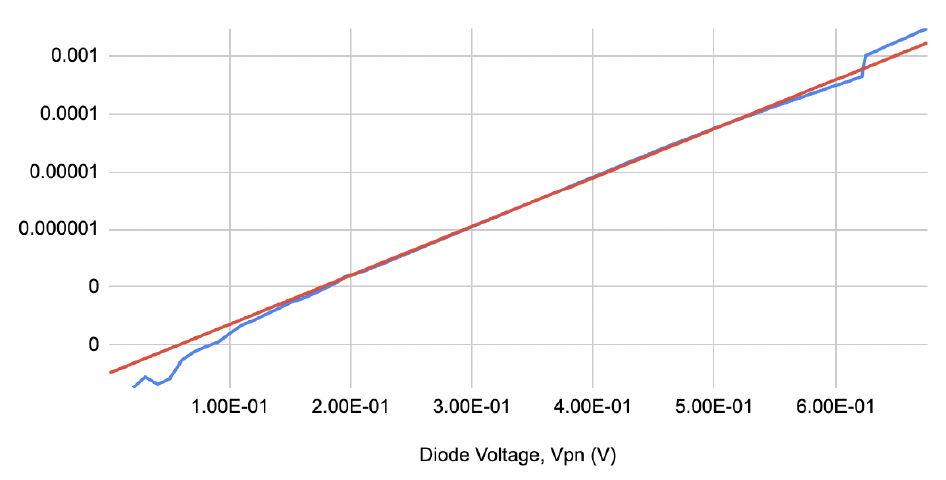
\includegraphics[width=0.95\textwidth]{q3_plot.png}
    \caption{}
    \label{fig:colored-leds-23}
\end{figure}

\item Comment on the values of $I_S$ and $n$ that yield the best
fit to the data. How do your values compare with those given in
the diode manufacturer data sheets? Include percent error. ($I_S$
can be found under reverse current (remember that $|I_R|\approx|
I_S|$), and $n$ should be about 2.3.)

- $Rs: (1.21 - 0.5) / 0.5 = 140\%$ error


- $Is: (5.2e-9 - 4e-9) / 4e-9 = 30\%$ error


- $n: (1.95 - 2.3) / 2.3 = 15.2\%$ 

The measured ideality factor of 1.95 indicates that the diode's behavior 
in real-world conditions deviates from the ideal case. For a 
near-ideal diode, the ideality factor would be closer to 1.

\end{enumerate}
\newpage
\section{Extension}
\end{document}